%%%%%%%%%%%%%%%%%%%%%%%%%%%%%%%%%%%%%%%%%%%%%%%%%%%%%%%%%%%%%%%%%%%%%%%%%%%%%%%%%%%%%%%%%%%%
%% DOCUMENT CLASS
%%%%%%%%%%%%%%%%%%%%%%%%%%%%%%%%%%%%%%%%%%%%%%%%%%%%%%%%%%%%%%%%%%%%%%%%%%%%%%%%%%%%%%%%%%%%
\documentclass[draft,11pt]{ucthesis}
%\documentclass[UC]{gcthesis}
%\documentclass[GC,twoside]{jdcthesis}

%%%%%%%%%%%%%%%%%%%%%%%%%%%%%%%%%%%%%%%%%%%%%%%%%%%%%%%%%%%%%%%%%%%%%%%%%%%%%%%%%%%%%%%%%%%%
%% DOUBLE SPACING
%%%%%%%%%%%%%%%%%%%%%%%%%%%%%%%%%%%%%%%%%%%%%%%%%%%%%%%%%%%%%%%%%%%%%%%%%%%%%%%%%%%%%%%%%%%%
%\def\dsp{\def\baselinestretch{2.0}\large\normalsize}
%\dsp

%%%%%%%%%%%%%%%%%%%%%%%%%%%%%%%%%%%%%%%%%%%%%%%%%%%%%%%%%%%%%%%%%%%%%%%%%%%%%%%%%%%%%%%%%%%%
%% DEFINITIONS OF SYMBOLS, FUNCTIONS
%%%%%%%%%%%%%%%%%%%%%%%%%%%%%%%%%%%%%%%%%%%%%%%%%%%%%%%%%%%%%%%%%%%%%%%%%%%%%%%%%%%%%%%%%%%%
%%%%%%%%%%%%%%%%%%%%%%%%%%%%%%%%%%%%%%%%%%%%%%
% THIS FILE CONTAINS DEFINITIONS AND COMMANDS
%%%%%%%%%%%%%%%%%%%%%%%%%%%%%%%%%%%%%%%%%%%%%%

%% Import useful packages.
%\usepackage{times}
%\usepackage{amsmath}                           	% for 'case'
%\usepackage{amsthm}                           	% for theorems and proofs
%\usepackage{mathrsfs}                          	% script math font
%\usepackage{url}                               	% allow use of URLs
%\usepackage{latexsym}                           % some math symbols, like \Box
%\usepackage{pseudocode}                         % for pseudocode environment
%\usepackage{subfigure}                           % allow use of subfigures

%% figure path
%\newif\ifpdf \ifx\pdfoutput\undefined
%\pdffalse
%\usepackage[dvips]{graphicx}
%\DeclareGraphicsExtensions{.eps,.epsi}
%\else
%\pdfoutput=1
%\pdfcompresslevel=9
%\pdftrue
%\usepackage[pdftex]{graphicx}
%\DeclareGraphicsExtensions{.pdf}
%\fi
%\graphicspath{{figures/}}

%% set up theorem block definitions
%\newtheorem{theorem}{Theorem}[section]
%\newtheorem{corollary}[theorem]{Corollary}
%\renewcommand{\thepseudonum}{\roman{pseudonum}}

%% quotations at beginning of chapters
%\newcommand{\myquote}[3]{
%\begin{flushright}
%\begin{minipage}[t]{#1}
%\itshape
%#3 \\
%\upshape
%\end{minipage}
%\\[-1mm]
%#2
%\end{flushright}
%\vspace{5mm}
%}


% Define some useful commands we will use repeatedly.
%\newcommand{\bfm}[1]{{\bf #1}}              % proper boldface for math environment
\newcommand{\bfm}[1]{{\mbox{\boldmath{$#1$}}}}               % proper boldface for math environment
%\newcommand{\bfm}[1]{{\boldsymbol{#1}}}               % proper boldface for math environment

\newcommand{\op}[1]{\mathcal{#1}}
%\newcommand{\vektor}[1]{{\bf #1}}
%\renewcommand{\vec}[1]{\bfm{#1}} % italicized boldface
\renewcommand{\vec}[1]{{\bf #1}}
\newcommand{\q}{\vec{q}} % coordinates
\newcommand{\p}{\vec{p}} % momenta
\newcommand{\z}{\vec{z}} % phase space point
\newcommand{\x}{\vec{x}} % general vector x
\newcommand{\M}{\bfm{M}} % diagonal mass matrix
\newcommand{\grad}{\nabla}
\newcommand{\timeavg}[1]{\overline{#1}}                    % time average over a trajectory
\newcommand{\T}{\mathrm{T}}                                % T used in matrix transpose
\newcommand{\tauarrow}{\stackrel{\tau}{\rightarrow}}       % the symbol tau over a right arrow
\newcommand{\expect}[1]{\langle #1 \rangle}                % <.> for denoting expectations over realizations of an experiment or thermal averages
\newcommand{\estimator}[1]{\hat{#1}}                       % estimator for some quantity from a finite dataset.
\newcommand{\code}[1]{{\tt #1}}

%\newcommand{\T}{\mathrm{T}}                                % T used in matrix transpose
%\newcommand{\tauarrow}{\stackrel{\tau}{\rightarrow}}       % the symbol tau over a right arrow
%\newcommand{\q}{\bfm{q}}
%\newcommand{\p}{\bfm{p}}
%\newcommand{\z}{\bfm{z}}
%\newcommand{\expect}[1]{\langle #1 \rangle}                % <.> for denoting expectations over realizations of an experiment or thermal averages
%\newcommand{\estimator}[1]{\hat{#1}}                       % estimator for some quantity from a finite dataset.
%%\newcommand{\bfm}[1]{\mbox{\boldmath{$#1$}}}               % proper boldface for math environment
%\newcommand{\bfm}[1]{{\bf #1}}
\newcommand{\program}[1]{\textsc{\lowercase{#1}}}  % Formatting to be used for program or package names.  This uses tiny 


\newcommand{\bra}[1]{\langle #1|}                          % Dirac bra <.|
\newcommand{\ket}[1]{|#1\rangle}                           % Dirac ket |.>
\newcommand{\braket}[2]{\langle #1|#2\rangle}              % Dirac bra-ket <.|.>

\newcommand{\oparg}{\:\cdot\:}           % argument of an operator
\newcommand{\set}[1]{\mathcal{S}_{#1}}           % argument of an operator



% Define mychapter
\newcommand{\mychapter}[1]{\chapter{#1}}

%%%%%%%%%%%%%%%%%%%%%%%%%%%%%%%%%%%%%%%%%%%%%%%%%%%%%%%%%%%%%%%%%%%%%%%%%%%%%%%%%%%%%%%%%%%%
%% PACKAGES
%%%%%%%%%%%%%%%%%%%%%%%%%%%%%%%%%%%%%%%%%%%%%%%%%%%%%%%%%%%%%%%%%%%%%%%%%%%%%%%%%%%%%%%%%%%%

% We will be using PDF figures and generating PDF output.
\pdfoutput=1
\pdfcompresslevel=9
\usepackage[pdftex]{graphicx}
\DeclareGraphicsExtensions{.pdf}

%\usepackage{graphicx}                   % graphic extended
\usepackage{cite}                       % to compress citations [1,2,3] -> [1-3], call it before babel 
                                        % (useless with hyperref)

%% Import useful packages.
\usepackage{times}
\usepackage{amsmath}                           	% for 'case'
\usepackage{amsthm}                           	% for theorems and proofs
\usepackage{mathrsfs}                          	% script math font
\usepackage{url}                               	% allow use of URLs
\usepackage{latexsym}                           % some math symbols, like \Box
\usepackage{pseudocode}                         % for pseudocode environment
\usepackage{subfigure}                           % allow use of subfigures
\usepackage{latexsym}                           % some math symbols, like \Box
\usepackage{multirow}
\usepackage{rotating}

%% figure path
%\newif\ifpdf \ifx\pdfoutput\undefined
%\pdffalse
%\usepackage[dvips]{graphicx}
%\DeclareGraphicsExtensions{.eps,.epsi}
%\else
%\pdfoutput=1
%\pdfcompresslevel=9
%\pdftrue
%\usepackage[pdftex]{graphicx}
%\DeclareGraphicsExtensions{.pdf}
%\fi
%\graphicspath{{figures/}}

%% set up theorem block definitions
%\newtheorem{theorem}{Theorem}[section]
%\newtheorem{corollary}[theorem]{Corollary}
%\renewcommand{\thepseudonum}{\roman{pseudonum}}

%% quotations at beginning of chapters
%\newcommand{\myquote}[3]{
%\begin{flushright}
%\begin{minipage}[t]{#1}
%\itshape
%#3 \\
%\upshape
%\end{minipage}
%\\[-1mm]
%#2
%\end{flushright}
%\vspace{5mm}
%}
% DOUBLE-SPACE
% \baselinestretch{2.0}\large\normalsize

%%%%%%%%%%%%%%%%%%%%%%%%%%%%%%%%%%%%%%%%%%%%%%%%%%%%%%%%%%%%%%%%%%%%%%%%%%%%%%%%%%%%%%%%%%%%
\begin{document}

%%%%%%%%%%%%%%%%%%%%%%%%%%%%%%%%%%%%%%%%%%%%%%%%%%%%%%%%%%%%%%%%%%%%%%%%%%%%%%%%%%%%%%%%%%%%
%% DECLARATIONS FOR FRONT MATTER
%%%%%%%%%%%%%%%%%%%%%%%%%%%%%%%%%%%%%%%%%%%%%%%%%%%%%%%%%%%%%%%%%%%%%%%%%%%%%%%%%%%%%%%%%%%%
\begin{frontmatter}

\title{Master equation models of macromolecular dynamics from atomistic simulation}
\author{John D. Chodera}
\degreeyear{2006}
\degreesemester{Fall}
\degree{Doctor of Philosophy}
\chair{Professor Ken A. Dill}
\othermembers{Professor Vijay S. Pande\\
Professor Matthew P. Jacobson}
\numberofmembers{3}
%\prevdegrees{B.S. (California Institute of Technology) 1999}
\field{Biophysics}
\campus{San Francisco}

\maketitle
%\approvalpage
\copyrightpage

%%%%%%%%%%%%%%%%%%%%%%%%%%%%%%%%%%%%%%%%%%%%%%%%%%%%%%%%%%%%%%%%%%%%%%%%%%%%%%%%%%%%%%%%%%%%
%% DEDICATION
%%%%%%%%%%%%%%%%%%%%%%%%%%%%%%%%%%%%%%%%%%%%%%%%%%%%%%%%%%%%%%%%%%%%%%%%%%%%%%%%%%%%%%%%%%%%
\begin{dedication}
\null\vfil
{\large
\begin{center}
Dedicated to the memory of Peter A. Kollman,\\\vspace{12pt}
whose unbounded enthusiasm for the field of biomolecular simulation was an inspiration.
 
\end{center}}
\vfil\null
\end{dedication}

%%%%%%%%%%%%%%%%%%%%%%%%%%%%%%%%%%%%%%%%%%%%%%%%%%%%%%%%%%%%%%%%%%%%%%%%%%%%%%%%%%%%%%%%%%%%
%% ACKNOWLEDGEMENTS
%%%%%%%%%%%%%%%%%%%%%%%%%%%%%%%%%%%%%%%%%%%%%%%%%%%%%%%%%%%%%%%%%%%%%%%%%%%%%%%%%%%%%%%%%%%%
\begin{acknowledgements}
% Acknowledge:
% - Julie Ransom
% - Bill Swope (de facto thesis advisor)
% - Ken Dill (thesis advisor)
% - Libusha (my ethical and scientific guide)
% - Peggy (for many years of fun)
% - My parents
% - Darby the cat (for putting up with me while doing this whole Ph.D. thing)
% - John Prentice (freelance physicist extraordaire)
% - Terry Lang (for being a scientific partner in crime)
% - The Dill lab (esp. Vince Voelz, Justin Bradford, Banu, and Kings)
% - The Biophysics/BMI/CCB kids (esp. Terry Lang, Mike Kim, Michael Reese)
% - Jerry Solomon and David Liney (for setting me on this path in the first place)
% - Jed Pitera (I seem to be following him around)
% - Vageli (who can actually solve problems)
% - Vijay / Nina
% - John Prentice
% - Peter Kollman
% - Lillian Chong
% - Del Tomeoni

No scientist works in a vacuum.
The scientific output of each individual is shaped to no small degree by those who have touched their lives deeply.
This dissertation is no exception.
I am indebted to so many people for their contributions to this work through direct and indirect means that it is not possible to name them all here, but I will try to touch on a few whose omission would certainly be a great injustice.

I thank the following people, not in order of importance, but rather mostly in order of appearance:
My mother, who taught me to read;
my father, who first showed me that it is possible to understand how the world around us works;
my constant childhood friend and mentor Delfo Tomeoni, who instilled within me the joy of finding things out;
Jr-Gang Cheng, who somehow recognized the seeds of an actual scientist within me while I was still a green-around-the-ears undergraduate, and taught me how to hold a pipetman;
Jerry Solomon and David Liney, who introduced me to protein folding, the problem that would consume much of my waking thoughts for the next ten years, and to the computational tools that could be used to understand it;
Peggy Gabriel, who made all those undergraduate years a lot more fun;
Peter Kollman, whose booming voice echoing through the hallways as he excitedly talked about free energy calculations I can still recall today;
Lillian Chong, my first rotation advisor, for ``showing me the ropes'' with AMBER and molecular dynamics simulation, whom I was delighted to have the chance to work with again at IBM;
Ken Dill, whose gentle guidance has made my graduate career a wonderful experience, and whose clarity of insight helped me develop a much deeper understanding of statistical mechanics;
the Dill lab crew, especially Banu Ozkan, whose work inspired my course in this thesis, Larry Schweitzer for keeping everything running so smoothly, and my classmates, Justin Bradford, Vincent Voelz, and Byoung-Chul Lee;
Bill Swope, whose scientific enthusiasm, attention to detail, and thoroughness I have come to greatly appreciate, and whom, along with Jed Pitera, I had the privilege to work with on body of work this dissertation encompasses;
Libusha Kelly for being my constant scientific and ethical sounding board, someone I can always count on to put me in my place when I screw up, and without whose constant encouragement this dissertation would have never been finished;
Nina Singhal and Vijay Pande, whom it has been my pleasure to work with throughout much of this dissertation;
Matt Jacobson, for always keeping his office door open, which let to numerous enjoyable and enlightening scientific discussions;
the Brass at UCSF kids, especially Alvin Mok, Brian Fife, Ann Wehman, Nick Endres, Terry Lang, and Ian Harwood, for ensuring there was at least \emph{one} night a week I wasn't working;
the Biophysics/BMI/CCB kids, especially Terry Lang, Michael Kim, and Michael Reese, for making science a whole lot of fun;
and finally, but perhaps most importantly, Julie Ransom, the benevolent shepherd of the Biophysics program, without whose tireless efforts I would surely be destitute, lying in a ditch somewhere in Tijuana, clutching a cheap bottle of bourbon. 

\begin{center}
$\bfm{\cdots}$
\end{center}

My thesis committee, consisting of Ken Dill (chair), Matt Jacobson, and Vijay Pande, deserves special thanks for reviewing this dissertation.  
The text of Chapter 2 largely contains material to appear in \emph{Journal of Chemical Theory and Computation}.
Chapter 3 contains material to appear in \emph{Multiscale Modeling and Simulation}.
Chapter 4 contains material to be submitted to the \emph{Journal of Physical Chemistry B}.
In these three chapters, co-authors made the following contributions: Bill Swope aided in the development of the theory and the interpretation of data and helped write the manuscript, and Jed Pitera participated in discussions and provided code upon which the parallel tempering simulation code is based.
Chaok Seok also contributed to development of some of the early theoretical development for Chapter 2, and implemented some early test code.
Ken Dill supervised the research that produced these chapters.
Chapter 5 contains material to be submitted to the \emph{Journal of Chemical Physics}.
There, Nina Singhal and I cowrote the manuscript with the assistance of Bill Swope, and Nina was responsible for the majority of the application of the algorithm to the various test systems and interpretation of the results.
Both Ken Dill and Vijay Pande supervised the research that produced this chapter.

\end{acknowledgements}

%%%%%%%%%%%%%%%%%%%%%%%%%%%%%%%%%%%%%%%%%%%%%%%%%%%%%%%%%%%%%%%%%%%%%%%%%%%%%%%%%%%%%%%%%%%%
%% ABSTRACT
%%%%%%%%%%%%%%%%%%%%%%%%%%%%%%%%%%%%%%%%%%%%%%%%%%%%%%%%%%%%%%%%%%%%%%%%%%%%%%%%%%%%%%%%%%%%
\begin{abstract}
Abstract goes here.

%The master equation formalism is a powerful tool for describing the dynamics of a system whose dynamics can be characterized by a discrete-state, continuous-time Markov process.  
%The evolution of experimentally measurable dynamical observables can be computed and compared with experiment.  
%Dynamical information not directly accessible to experiment, such as folding pathways, transiently populated conformations, and mean first passage times, can also be easily obtained.  
%We are investigating methods for constructing master equation models of protein dynamics from realistic molecular mechanics models, where metastable subsets of conformation space are represented by discrete states.  
%We believe this approach will provide a useful bridge between the short timescales accessible by molecular dynamics simulation and the long timescales accessible by experiment.

%In order to construct discrete-state, continuous-time master equation models from molecular mechanics models of proteins, two essential components are necessary: 
%(1) a method of dividing up configuration space into metastable subsets, and (2) a way of efficiently computing transition rates between these subsets.  
%In the past year, we have made significant progress on (2).  
%Parallel tempering (or replica-exchange among temperatures) molecular dynamics simulations are used to efficiently explore conformational energy landscapes and generate ensembles of short trajectory segments at several temperatures.  
%We have extended histogram reweighting methods to allow dynamical observables, such as transition probabilities between conformational subsets, to be optimally estimated at any temperature in the range spanned by the replica temperatures.  
%This allows efficient estimation of transitions that are rare at low temperatures.
%Coupled with an alogrithm to partition configuration space, we will be able to construct master equation models at various temperatures, replicating popular experimental nonequilibrium conditions, such as T-jump unfolding.

%My current research focuses on understanding common features of protein folding mechanisms and protein dynamics by the use of atomistic simulations.  
%Though molecular dynamics trajectories can only reach relatively short timescales, through the use of many short trajectories generated by parallel computers, we can build meso-scale models of conformational dynamics through the construction of Markov models representing transitions between metastable conformational substates. 
%Recent results indicate that this approach is able to accurately describe the long-time dynamics of small peptides in explicit solvent.

%In order to develop a detailed understanding of biomolecular dynamics and protein folding kinetics, we need to characterize the statistical dynamics of the molecular system over times that are long compared to the timescales accessible by molecular dynamics simulation. 
%Luckily, due to the hierarchical nature of the energy landscape and the presence of a viscous solvent, a natural separation of timescales makes it possible to model dynamics as a series of infrequent transitions between metastable conformational substates. 
%If phase space is fragmented into a sufficient number of conformational substates, these interstate transitions can be well characterized by large numbers of molecular dynamics simulations in parallel or by importance sampling techniques. 
%The resulting model is a discrete-state, continuous-time Markov process, where we can make use of the master equation formalism for which there exist powerful tools for the study of dynamical behavior. 
%We demonstrate that such a model accurately describes the dynamics of a small solvated peptide system and discuss our recent work in developing efficient multistage algorithms for construction of these models from explicit-solvent molecular dynamics simulations.


\abstractsignature
\end{abstract}

%%%%%%%%%%%%%%%%%%%%%%%%%%%%%%%%%%%%%%%%%%%%%%%%%%%%%%%%%%%%%%%%%%%%%%%%%%%%%%%%%%%%%%%%%%%%
%% TABLES OF CONTENTS, LISTS OF FIGURES AND TABLES
%%%%%%%%%%%%%%%%%%%%%%%%%%%%%%%%%%%%%%%%%%%%%%%%%%%%%%%%%%%%%%%%%%%%%%%%%%%%%%%%%%%%%%%%%%%%
\tableofcontents
\listoffigures
\listoftables

\end{frontmatter}

%%%%%%%%%%%%%%%%%%%%%%%%%%%%%%%%%%%%%%%%%%%%%%%%%%%%%%%%%%%%%%%%%%%%%%%%%%%%%%%%%%%%%%%%%%%%
%% TABLE OF SYMBOLS
%%%%%%%%%%%%%%%%%%%%%%%%%%%%%%%%%%%%%%%%%%%%%%%%%%%%%%%%%%%%%%%%%%%%%%%%%%%%%%%%%%%%%%%%%%%%
%%%%%%%%%%%%%%%%%%%%%%%%%%%%%%%%%%%%%%%%%%%%%%%%%%%%%%%%%%%%%%%%%%%%%%%%%%%%%%%%%%%%%%%%%%%%%
%% TABLE OF SYMBOLS
%%%%%%%%%%%%%%%%%%%%%%%%%%%%%%%%%%%%%%%%%%%%%%%%%%%%%%%%%%%%%%%%%%%%%%%%%%%%%%%%%%%%%%%%%%%%

\begin{table*}[p]
\caption{{\bf Notation.}}
% :TODO: Change this to {lp{somewidth}}.
\begin{tabular}{ll}
\hline
%%%%%%%%%%%%%%%%%%%%%%%%%%%%%%%%%%%%%%%%%%%%%%%%%%%%%%%%%%%%%%%%%%%%%%%%%%%%%%%%%%%%%%%%%%%%
% GENERAL NOTATION
%%%%%%%%%%%%%%%%%%%%%%%%%%%%%%%%%%%%%%%%%%%%%%%%%%%%%%%%%%%%%%%%%%%%%%%%%%%%%%%%%%%%%%%%%%%%
\multicolumn{2}{l}{\bf General notation} \\
$\expect{A}_\beta$ & configuration space average in the canonical ensemble at inverse temperature $\beta$ \\
$\expect{A}$ & mathematical expectation, such as average over repeated realizations of an experiment \\
$\timeavg{A}$ & time average over a trajectory \\
$\estimator{A}$ & estimator of $\expect{A}$ \\
$\delta^2 \estimator{A}$ & squared uncertainty in $\estimator{A}$ \\
%%%%%%%%%%%%%%%%%%%%%%%%%%%%%%%%%%%%%%%%%%%%%%%%%%%%%%%%%%%%%%%%%%%%%%%%%%%%%%%%%%%%%%%%%%%%
% VECTORS
%%%%%%%%%%%%%%%%%%%%%%%%%%%%%%%%%%%%%%%%%%%%%%%%%%%%%%%%%%%%%%%%%%%%%%%%%%%%%%%%%%%%%%%%%%%%
\multicolumn{2}{l}{\bf Vectors} \\
$\bfm{q}$ & coordinates, $\bfm{q} \in \Re^{3N}$ \\
$\bfm{p}$ & momenta, $\bfm{q} \in \Re^{3N}$ \\
$\bfm{z}$ & phase space point $\bfm{z} = (\bfm{q}, \bfm{p})$, $\bfm{z} \in \Re^{6N}$ \\
%%%%%%%%%%%%%%%%%%%%%%%%%%%%%%%%%%%%%%%%%%%%%%%%%%%%%%%%%%%%%%%%%%%%%%%%%%%%%%%%%%%%%%%%%%%%
% PARAMETERS AND VARIABLES
%%%%%%%%%%%%%%%%%%%%%%%%%%%%%%%%%%%%%%%%%%%%%%%%%%%%%%%%%%%%%%%%%%%%%%%%%%%%%%%%%%%%%%%%%%%%
\multicolumn{2}{l}{\bf Parameters and variables} \\
$U$ & potential energy \\
$k_B$ & Boltzmann's constant \\
$T$ & temperature \\
$\beta$ & inverse temperature $1/(k_B T)$ \\
$M$ & number of potential energy bins \\
$U_m$ & potential energy at center of bin $m$ \\
$\Delta U$ & width of potential energy bins \\
$K$ & number of simulations or replicas \\
$N_k$ & number of snapshots from simulation $k$ \\
$\tau$ & integrated autocorrelation time \\
$g$ & statistical inefficiency \\
$w_k$ & weights for combining estimates from different simulations \\
$f_k$ & dimensionless Helmholtz free energy of simulation $k$ \\
%%%%%%%%%%%%%%%%%%%%%%%%%%%%%%%%%%%%%%%%%%%%%%%%%%%%%%%%%%%%%%%%%%%%%%%%%%%%%%%%%%%%%%%%%%%%
% FUNCTIONS
%%%%%%%%%%%%%%%%%%%%%%%%%%%%%%%%%%%%%%%%%%%%%%%%%%%%%%%%%%%%%%%%%%%%%%%%%%%%%%%%%%%%%%%%%%%%
\multicolumn{2}{l}{\bf Functions} \\
$A({\bf q})$ & phase space observable (depends only on coordinates) \\
$U({\bf q})$ & potential energy \\
$\Omega(U)$ & density of states for potential energy \\
$\psi_m(U)$ & indicator function for energy bin $m$ \\
$P_m(\beta)$ & probability of energy bin $m$ at inv. temperature $\beta$ \\
$Z(\beta)$ & canonical partition function at inv. temperature $\beta$ \\
$p_m(\beta)$ & unnormalized probabilities for different energy levels at inverse temperature $\beta$ \\
%%%%%%%%%%%%%%%%%%%%%%%%%%%%%%%%%%%%%%%%%%%%%%%%%%%%%%%%%%%%%%%%%%%%%%%%%%%%%%%%%%%%%%%%%%%%
% DISCRETIZED FUNCTIONS
%%%%%%%%%%%%%%%%%%%%%%%%%%%%%%%%%%%%%%%%%%%%%%%%%%%%%%%%%%%%%%%%%%%%%%%%%%%%%%%%%%%%%%%%%%%%
\multicolumn{2}{l}{\bf Discretized functions} \\
$H_{m,k}$ & number of snapshots from replica $k$ with potential energy falling in bin $m$ \\
$\Omega_{m}^{(k)}$ & estimate of the density of states for energy bin $m$ from simulation or replica $k$ \\
%\multicolumn{2}{l}{\bf Timeseries data} \\
%${\bf q}_{kn}$ & coordinates of snapshot $n$ from simulation or replica $k$ \\
%$U_{kn}$ & potential energy of snapshot $n$ from simulation or replica $k$ \\
%$\beta_{kn}$ & inverse temperature of canonical ensemble from which snapshot $n$ and replica $k$ was generated \\
%$\psi_{m,kn}$ & value of the indicator function for potential energy bin $m$ for snapshot $n$ of replica $k$ \\
%$A_{kn}$ & value of the observable $A$ for snapshot $n$ of replica $k$ \\
%$w_{kn}$ & weight of snapshot $n$ of replica $k$ at the temperature of interest \\
%$B_{kn}$ & new observable defined as $w_{kn} A_{kn}$ \\
\hline
\end{tabular}
\end{table*}

%%%%%%%%%%%%%%%%%%%%%%%%%%%%%%%%%%%%%%%%%%%%%%%%%%%%%%%%%%%%%%%%%%%%%%%%%%%%%%%%%%%%%%%%%%%%
%% INTRODUCTION
%%%%%%%%%%%%%%%%%%%%%%%%%%%%%%%%%%%%%%%%%%%%%%%%%%%%%%%%%%%%%%%%%%%%%%%%%%%%%%%%%%%%%%%%%%%%
\chapter{Introduction}
%\mychapter{Introduction}
\label{chapter:introduction}

\section*{Perspective}

%\subsection*{Conformational dynamics in biology}

%Biological macromolecules are inherently dynamic molecular machines.
Conformational dynamics plays an integral role in the function of biological macromolecules.
Proteins, after translation by the ribosome, rapidly fold to well-defined native topologies that bring disparate chemical moieties together into a particular geometry, conferring the ability to perform chemical catalysis \cite{stryer:biochemistry}.
Errant misfolding can lead to aggregation and the formation of amyloid plaques, a phenomenon associated with diseases such as Alzheimer's, Parkinson's, and Creutzfeldt-Jacob (``Mad Cow'') Diseases \cite{dobson:nature:2003:misfolding}.
Once folded, excursions to partially unfolded states can expose proteins to proteolysis; to avoid this, some organisms appear to have evolved secreted proteases that are kinetically stable to maintain competitive advantage in harsh extracellular environments \cite{jaswal:jmb:2005:alpha-lytic}.
Conformational changes of folded proteins can be critical for protein \cite{hirose:molcell:2006} or substrate binding \cite{vandenhemel:jbc:2006} and catalytic function \cite{kern:science:2002,youngblood:jbc:2006a,boehr:2006a}.
Together with order-disorder transitions \cite{dyson:nat-rev-mol-cell-biol:2005}, ordered sequences of conformational changes are integral to the transformation of chemical energy into mechanical work by motor proteins \cite{kambara:jbc:2006,schulten:structure:2006} or the reverse by ATP synthases \cite{noji:nature:1997}.
Binding or post-translational modification events far from the active site can modulate the activity of proteins through allosteric effects, which involve poorly understood structural or dynamical changes transmitted through largely unknown mechanical or electrostatic pathways \cite{frauenfelder:pnas:2001,changeux:2005a,maki:jbc:2006a}.
Slow prolyl \emph{cis-trans} isomerization dynamics can be used as a molecular timer \cite{eckert:nsmb:2005:prolyl-isomerization-molecular-timer}, which can be modulated by phosphorylation events for signaling purposes \cite{wulf:ncb:2005:phosphorylation-specific-prolyl-isomerization}.
Ion channel gating, an inherently stochastic kinetic process involving conformational switching between multiple conductance states \cite{mannuzzu:science:1996,cordero-morales:nsmb:2006:gating-of-KcsA}, can be modulated by transmembrane voltage \cite{bezanilla:physiol-rev:2000,cordero-morales:nsmb:2006:KcsA-voltage-gating}, ligand binding at allosteric sites \cite{dably-brown:curr-topics-med-chem:2006:Kv7-modulators}, temperature \cite{tominaga:jneurobiol:2004:thermosensation}, mechanical pressure \cite{perozo:nrmcb:2006:gating-mechanosensitive-channels}, and phosphorylation \cite{levitan:annu-rev-physiol:1994}, and undergo time-dependent inactivation \cite{demo:neuron:1991}.
The conformational plasticity of RNA no doubt contributes to its many characterized biological roles in information transmission \cite{ogle:science:2001,sanbonmatsu:biochimie:2006}, binding \cite{ha:pnas:1999}, and catalysis \cite{zhuang:science:2002:structural-dynamics-ribozyme-function,ke:nature:2004:ribozyme-catalysis-conformational-switch}.
In each of these cases, conformational dynamics plays an integral role in macromolecular folding, assembly, function, and regulation, and a detailed description of this dynamical behavior is likely critical to achieving an understanding of the corresponding biological phenomena.

Structural biology has proven to be a valuable tool for the study of these machines.
Structural studies, especially X-ray crystallography and nuclear magnetic resonance (NMR) spectroscopy, allow the determination of experimentally-derived structural models which can aid the formulation of hypotheses about function, mechanism, and disease.
However, these methods have generally been limited to producing \emph{static} pictures of macromolecules.
While attempts have been made to relate crystallographic Debye-Waller factors (``B-factors'') to biologically relevant conformational fluctuations \cite{bahar:folding-design:1997,kondrashov:biophysj:2006}, this interpretation is complicated by the fact that the majority of these crystals are cryogenically cooled before the collection of scattering data to temperatures well below the glass transition temperature \cite{weik:acta-cryst-d:2001} over times sufficiently long to allow for significant structural rearrangement \cite{kriminski:2003a}.
Additionally, the presence of crystallographic and non-crystallographic neighbors, salts, and cosolvents, and binding partners in a crystal lattice suggests the relevance of information on dynamics or heterogeneity obtained from these data should be treated as suspect unless proven otherwise by extensive comparison with experimental data under more biological conditions.
In principle, NMR provides information on both conformational heterogeneity and dynamics in solution, but the difficulty of interpreting this data, coupled with the small number of experimental observations per residue, has made extraction of anything but average structures (a surprisingly robust problem \cite{tang:1999a}) difficult, though work continues on improving this situation \cite{rieping:2005a,lindorff-larsen:2005a}.
Standard NMR refinement protocols \cite{nilges:protein-engineering:1988} produce ensembles of structures, but the resulting ensemble may not represent conformational heterogeneity; in fact, assumptions that the data comes from a single conformation ensure this cannot be the case.
As a result, the ensemble is composed of \emph{virtual} structures that may not exist in solution with high probability \cite{jardetzky:biochimica-et-biophysica-acta:1980}.
These structures simply represent minima of the target function, a sum of a least-squares error function with experiment and a molecular mechanics forcefield.
Additionally, the conformational diversity observed in these ensembles cannot easily be determined to be due to conformational averaging in solution or a lack of sufficient experimental restraints, but is usually an underestimate of the true diversity that is possible for an ensemble that satisfies the NMR restraints on average \cite{spronk:j-biomol-nmr:2003}.
Despite these problems, these methods have provided structural models which have been tremendously useful for the generation of models and experimentally testable hypotheses, rapidly accelerating our ability to understand biological function and mechanism.

In order to more directly probe conformational heterogeneity and dynamics, a number of other biophysical techniques have been developed.
Certain NMR experiments can provide information on picosecond and nanosecond timescales \cite{wand:chem-rev:2006}, but the amount of information that can be extracted and its interpretation has proven even more difficult that the extraction of information about conformational heterogeneity.
F\"{o}rster resonance energy transfer (FRET), in which two fluorescent probe molecules with overlapping emission and absorbance spectra are covalently attached to different groups of the molecule, allows for determination of the interprobe distance from the observed fluorescence emission.
Other spectroscopic assays that do not require covalent modification, such as UV circular dichroism (CD), Fourier transform infrared spectroscopy (FTIR), and tryptophan fluorescence, also provide sensitive probes of different aspects of molecular structure and environment, though the interpretation of these spectra is often difficult and the information that can be extracted limited.
Recent advances, such as two-dimensional infrared spectroscopy (2DIR) \cite{khalil:2003a} can provide more information at the expense of sacrificed time resolution, allowing some individual chemical moieties to be resolved.

These spectroscopic probes can be employed to study either equilibrium thermodynamics over a range of conditions (such as temperature or denaturant concentration) or kinetics, in which relaxation from nonequilibrium initial conditions or equilibrium fluctuations are observed.
In \emph{ensemble} experiments, in which a solution of many macromolecules is monitored at equilibrium or after a rapid perturbation (such as rapid heating of the solvent with a short laser pulse \cite{gruebele:1998a}), high time resolution is possible because signal is collected from many molecules.
However, due to the presence of large numbers of molecules, these experiments can only provide information about the average spectroscopic signal over the ensemble --- information on heterogeneity within the ensemble is lost.
As a result, much effort has recently been focused on the development of \emph{single molecule} experiments, which can provide information about the heterogeneity of both equilibrium distributions and individual microscopic trajectories.
To obtain equilibrium distributions, it is sufficient to work with solutions that are sufficiently dilute such that it is unlikely that more than one molecule is in the region under spectroscopic surveillance at any one time.
To observe dynamic trajectories, however, these molecules must be prevented from diffusing away from the observation area.
This is typically done through the use of covalently attached or noncovalently-bound molecular linkers tethered to the glass slide, or by encapsulation in immobilized vesicles \cite{rhoades:2004a}.
However, to gather sufficient numbers of photons to give a reasonable signal-to-noise ratio, time resolution must be sacrificed, leading to experimental time resolution of milliseconds for single-molecule experiments, rather than the nanosecond resolution achievable by ensemble experiments.

Because of these limitations, there is still an unmet desire to observe the dynamics of individual molecules with high time resolution and in atomic detail.
Clearly, further advances in engineering and ongoing development of new methods will continue to push the boundaries of what is experimentally observable.
However, fundamental limitations, such as the tradeoff between time resolution and information about heterogeneity in ensemble and single-molecule experiments above, and the ability to observe only spectroscopically active changes mean there is only so much information that can be expected from experimental methods.

Additionally, there appears to be a lack of consensus regarding the fundamental physical nature of the experimental observations and how to interpret them, or even how to summarize them in terms of sufficient statistics.
The temporal signal from ensemble kinetics experiments, for example, has been variously fit to exponentials \cite{eaton:jpcb:2000}, sums of exponentials \cite{eaton:biochem:1997,munoz:1997a,steinbach:biophys-j:2002,yang:2004c}, and so-called \emph{stretched exponentials} \cite{gruebele:pnas:2005}.
The presence of a \emph{burst phase} means that there is immediate and unexplained loss of spectroscopic signal in the \emph{dead time} of the experiment, immediately after the perturbation (e.g. stopped flow mixing or laser temperature-jump \cite{gruebele:1998a}).
A statistical mechanical framework which would permit explanation of all of these observed phenomena and at least provide a physical functional form of the resulting observations, and ideally a connection with the actual microscopic dynamics, would be beneficial.

With the advent of the modern microcomputer, a new kind of experiment became possible, in which the detailed atomic motions of the macromolecule and its environment were simulated given a suitable model for the interatomic forces.
These molecular dynamics simulations promised the ability to model molecular processes in atomic detail and high time resolution, providing the microscopic detail missing from single-molecule or ensemble experiments mentioned above.
However, gathering insight into biological processes from these trajectories faces several challenges.
On contemporary workstations, molecular dynamics simulations with explicit representations of the solvent environment can reach simulation times generally limited to tens of nanoseconds --- far shorter than even the fastest characterized folding protein times of microseconds. 
While current-generation supercomputers, with several moths of massively parallel computation, can reach timescales of up to 10 $\mu$s for small proteins \cite{germain:2005a}, a \emph{single} long trajectory in which only one event of interest occurs (e.g. a protein folding event) does not give much information about an inherently stochastic and heterogeneous process.
By contrast, distributed computing projects \cite{pande:2000a,pande:2002a} offer the ability to produce many thousands of short trajectories, but there exists the danger that the mechanism by which the event of interest occurs (e.g. protein folding) may be biased, in that the mechanism at short times may differ from the mechanism at long times, where the bulk of events might occur \cite{fersht:2002a,marianayagam:2005a}.

The forcefields commonly employed in molecular dynamics simulations are also known to be vast simplifications of the actual physical interactions, neglecting some contributions, such as polarizability, completely.
Comparison with experiment to assess the severity of these omissions, however, is frustrated by the fact that ensemble experiments provide information about averages over many macromolecules while simulations typically consider only single molecules. % Redundant?
On the other hand, comparison with single molecule experiments is difficult due to the low time resolution of the experimental data and the difficulty of generating sufficiently long simulation trajectories.

As a result, the accuracy with which current-generation forcefields can model biomolecular kinetic processes is still largely unknown.
What is needed is some way to bridge the \emph{timescale gap} between short atomistic simulations of single molecules and long experimental observations of ensembles of molecules.
Ideally, this could be done through the construction of a statistical model that contains information about the heterogeneity by which the dynamical processes of interest may occur.
This model would have to be constructed from relatively short simulations of single molecules, and yet describe the stochastic dynamics of either a single molecule or a (noninteracting) ensemble of molecules over much longer times.

%\subsection*{Conformational dynamics and metastable states}

% JDC: Restrict citations here to work that came before I started on this thesis?

Fortunately, there is good evidence that the fundamental physical nature of intramolecular interactions makes it is possible to construct simple stochastic models of macromolecular dynamics.
Pioneering work by Christof Sch\"{u}tte, Huisinga, and coworkers at the Zuse Institute of Berlin \cite{schuette:1999a,schuette-thesis,fischer-thesis,deuflhard:2000a,galliat:2000a,huisinga-thesis,galliat-thesis,fischer-thesis} (and later Weber and Kube \cite{weber-thesis:2006a,kube:2006a}), as well as independent work by Shalloway and coworkers \cite{shalloway:1996a,ulitsky:1998a,ulitsky:1999a,church:2001a}, and Berry and coworkers \cite{ball:1998b,despa:2001a,levy:2002a,despa:2003a}, proposed that macromolecules might exhibit behavior suggestive of long-lived \emph{metastable conformational states}. %  Double-check non-ZIB references
The dynamics of a system with strongly metastable states is characterized by long waiting times \emph{within} these states, punctuated by infrequent stochastic transitions \emph{between} states.

The existence of metastable states is a simple consequence of the presence of a separation of timescales between \emph{fast intrastate motion} and \emph{slow interstate motion}.
It is widely believed that the nature of the energy landscape of biomacromolecules is hierarchical \cite{ansari:1985a,bai:1989a,becker:1997a,levy:2001a,levy:2002a}.
Indeed, proteins are known to exhibit a wide dynamic range of timescales, from femtosecond bond vibration to nanosecond helix formation to microsecond or greater folding times.
% JDC: Libusha suggests making the following into a table.  It would be great to dig up references too.
%bonds vibrate with periods of tens of femtoseconds; water orientational relaxation occurs on picosecond timescales; contacts form on nanosecond timescales, and helices on tens or hundreds of nanoseconds; the fastest proteins fold in microseconds, but many fold much more slowly, in milliseconds; some conformational transitions, such as proline isomerizations, take place on many second timescales; kinetically trapped proteins have been found that have half-lives of years [CITE ALPHA-LYTIC]. 
The hierarchical nature of the energy landscape presents an intriguing possibility: If there are many gaps in the spectrum of timescales (as would be expected from a hierarchical landscape), rather than a continuum (which would have to have a continuous and relatively flat distribution of barrier heights), then it should be possible to construct \emph{many} models with different numbers of metastable states capable of describing conformational dynamics, each with a different spatial and temporal resolution.
These models need only be as detailed as necessary for describing the phenomena of interest, simplifying the process of interpreting experiments, understanding dynamics, and extracting chemical insight.

The resulting stochastic model, produced by coarse-graining conformation space into metastable states, is a discrete-state, continuous-time \emph{master equation model}, in which transitions between states are described by first-order kinetics governed by a \emph{rate matrix}.
As will be discussed at length, the simplicity of the model comes at the cost of incurring a coarse-graining in time; temporal resolution is lost because conformational dynamics occurring on timescales comparable with motion \emph{within} states is omitted in the model.
Despite this, the master equation model possesses numerous benefits.
The entire statistical dynamics over times longer than some intrinsic \emph{internal equilibration time} is available, allowing the production of single-molecule trajectories or ensemble evolution experiments, as well as allowing direct comparison with nonequilibrium relaxation kinetics experiments, the computation of unobservable properties like $P_\mathrm{fold}$ \cite{du:1998a} that aid in the understanding of mechanism \cite{lenz:2004a}, and the summarization of primary events in kinetics processes such as folding, most notably seen in the work of Banu Ozkan and Ken Dill \cite{ozkan:2001a,ozkan:2002a}.


\section*{Synopsis}

% JDC: Note: The commented-out text ideals

%The aim of this dissertation is twofold.

%First, we develop a statistical mechanical framework for modeling macromolecular conformational dynamics as stochastic transitions between metastable states for use as both a conceptual theoretical model for thinking about dynamics, interpreting and deigning experiments (both computational and experimental), and constructing efficient simulation algorithms.
%This framework provides a rigorous connection between the master equation model, which is often treated as a purely phenomenological construct, and the classical statistical dynamics governing the evolution of macromolecular systems, and allows the necessary and sufficient conditions under which the model faithfully represents dynamics to be enumerated.

%Second, we build upon this framework by designing efficient algorithms for the construction of these stochastic models from atomistic molecular dynamics simulations in explicit solvent, in order to provide tools for the investigation of these dynamical processes and dynamics pictures from which experimental hypotheses can be generated.
%Just as structural models derived from X-ray or NMR data drove a revolution in biophysical and biochemical experimentation, these tools offer the possibility of generating models that are dynamical in nature, from which new insight into mechanistic models and experimental hypotheses may come.
%The eventual development of forcefields of sufficient accuracy to reliably model macromolecular interactions may even elevate molecular simulation to a  tool on par with and complementary to existing experimental methods.

%Chapter \ref{chapter:statistical-mechanics} contains a review the classical statistical mechanics describing the equilibrium and dynamical behavior of solvated biomacromolecular systems.
%Some readers may find this material elementary, but notation used throughout this dissertation is introduced.

%Chapter \ref{chapter:derivation-of-master-equation} presents the case for modeling macromolecular dynamics as a series of stochastic transitions between metastable states, and sets out the formal theory for deriving this model from the underlying statistical mechanics.
%One approach based on the eigenfunction expansion of the Liouvillean is sketched, as it is useful for providing insight into experiments and simulations, and a detailed derivation using the Mori-Zwanzig projection operator formalism is presented.
%Various properties of the resulting master equation model are enumerated, and a compendium of useful things that can easily be computed from it given.

%Chapter \ref{chapter:validation-of-master-equation} is concerned with how these models, once constructed from simulation data, can be validated to determine the timescale for emergence of Markovian behavior.
%An model system where dynamics of the model can be compared directly with numerous long simulations, terminally blocked alanine in explicit solvent, is introduced, and will be a recurring example used for illustrative purposes.

%Chapter \ref{chapter:automatic-state-decomposition} describes progress toward algorithms for the discovery of metastable states without prior knowledge of the relevant degrees of freedom.

%Chapter \ref{chapter:efficient-computation-of-transition-rates} focuses on the issue of efficiently computing transition probabilities between these states, once defined, and introduces the formalism of the \emph{transition energy density of states}. 
%Through this formalism, and exploiting an analogue of the weighted histogram analysis method, data from static equilibrium simulations, equilibrium trajectories, trajectories initiated from equilibrium distributions over the states, and trajectories harvested from transition path sampling simulations can be combined to obtain an optimal estimate of the transition probabilities and rates.
%Temperature-dependent transition probabilities and rates can also be obtained.

%Finally, Chapter \ref{chapter:automatic-construction-of-master-equation} suggests ways in which these pieces of technology might be combined to construct a multistage or iterative procedure for automatically constructing master equation models in an efficient manner given whatever structural data may be initially available.
%
%Two appendices provide a review of the derivation of the weighted histogram analysis method, which is exploited extensively in this thesis, and a primer on the calculation of statistical uncertainties from molecular simulations.

This thesis is organized as follows.
Chapter \ref{chapter:wham} contains a variant of the weighted histogram analysis method that can treat simulated and parallel tempering simulations, and estimate the statistical uncertainty in equilibrium averages computed from these simulations.
This was used extensively as a tool in subsequent work.
Chapter \ref{chapter:mastereqn-alanine-long-times} contains a manuscript which is to appear in the journal \emph{Multiscale Modeling \& Simulation} that introduces the Markov chain or master equation model and illustrates that a model constructed from short trajectories can describe the long-time statistical dynamics of terminally-blocked alanine in explicit solvent.
Chapter \ref{chapter:validation-of-master-equation} contains a manuscript to be submitted to the \emph{Journal of Physical Chemistry B} that is concerned with how these models, once constructed short trajectories, can be validated to determine the timescale for emergence of Markovian behavior.
Finally, Chapter \ref{chapter:automatic-state-decomposition} describes progress toward algorithms for the discovery of metastable states without prior knowledge of the relevant degrees of freedom, the final piece of the puzzle necessary for the construction of these models for biomolecules.



%%%%%%%%%%%%%%%%%%%%%%%%%%%%%%%%%%%%%%%%%%%%%%%%%%%%%%%%%%%%%%%%%%%%%%%%%%%%%%%%%%%%%%%%%%%%
%% CHAPTERS
%%%%%%%%%%%%%%%%%%%%%%%%%%%%%%%%%%%%%%%%%%%%%%%%%%%%%%%%%%%%%%%%%%%%%%%%%%%%%%%%%%%%%%%%%%%%
%\chapter{The statistical mechanics of macromolecular dynamics}
%\label{chapter:statistical-mechanics}
%\section{Modeling the macromolecular system}

Consider a biomacromolecule in a solvated environment under typical biological or experimental conditions.
Our interest lies in the conformational dynamics of this macromolecule.
We presume the system can be treated entirely within the realm of classical statistical mechanics for the following reasons:
\begin{enumerate}
  \item Because atomic nuclei are at least three orders of magnitude more massive than the electrons, the electronic degrees of freedom relax much more rapidly than the nuclei move, and can be considered as always occupying their ground state in the field of the nuclei.  
  This is the celebrated Born-Oppenheimer approximation \cite{born:1927a}.
  \item Quantized vibrations and zero-point energy effects are minimal due to the thermal kinetic energies under biological conditions\footnote{Comparison with experiment will occasionally still require correction terms to account for quantum effects that cannot be treated classicaly, such as quantized vibration effects, as in \cite{horn:jcp:2004}}.
  \item In restricting our consideration to conformational dynamics and not chemical reactions, we require that chemical bonds are neither broken nor formed.
  This ensures that we do not need to treat nuclear wavefunctions, as might be the case in enzyme-catalyzed hydrogen transfer reactions \cite{hammes-schiffer:acc-chem-res:2006}.
\end{enumerate}
The interatomic interactions can be completely described by some potential function $V(\q)$ that depends only on the Cartesian coordinates\footnote{We note that this exposition could be extended to allow the use of generalized coordinates and momenta, but this would necessitate the use of a Jacobian correction factor in the resulting phase space densities and partition functions.  Therefore, for simplicity, we leave this extension as an exercise to the reader, should it be necessary.} of the atomic nuclei $\q \in \Re^{3N}$.
This potential is sometimes termed a \emph{forcefield} due to the fact that it is the field whose negative gradient yields the instantaneous interatomic forces: \index{forcefield} \label{notation:force} \index{force}
\begin{eqnarray}
\bfm{F}(\q) &=& - \grad_{\q} V(\q) \label{equation:force-definition}
\end{eqnarray}
The exact form of the potential is not of interest here, but there are several popular \emph{molecular mechanics forcefields} in common use today, such as AMBER \cite{AMBER-parm94,AMBER-parm96,AMBER-gaff,duan:2003a}, CHARMM \cite{mackerell:jpcb:1998}, and GROMOS \cite{oostenbrink:j-comput-chem:2004}. \index{forcefield!molecular mechanics}

Although macromolecular crowding is known to have an effect on thermodynamics and conformational dynamics \cite{elcock:pnas:2003:crowding,chebotareva:biochem-moscow:2004:crowding,zhou:j-mol-recognit:2004:crowding,zhou:jbc:2004:crowding,volker:annu-rev-biophys-biomol-struct:2005,minton:j-cell-sci:2006}, and many macromolecules primarily exist in complexes or assemblies \cite{sali:nature:2003}, we restrict our consideration here to a single independent macromolecule\footnote{While the methods presented here may be extended to more complex systems of multiple interacting macromolecules and ligands, we restrict ourselves to consideration of a single macromolecule here, for simplicity.}. \index{crowding}
This situation corresponds to a solution of macromolecules sufficiently dilute such that each can be considered as independent or noninteracting, which may be the case in some, but not all, experiments.
Typically, the macromolecule is surrounded by a large amount of solvent (generally water) under near-atmospheric external pressures.
In biological systems, as well as many experiments, the salt concentration ensures that some mobile counterions will surround the macromolecule\footnote{Standard practice in molecular simulations is to add only the minimal number of individual counterions to bring the system to net neutrality.  This practice may result in an atypical effective salt concentration that is not representative of either \emph{in vitro} or \emph{in vivo} conditions.  As an example, a recent simulation of the trpzip2 hairpin \cite{pitera:2006a} employed a cubic simulation box (48 \AA)$^3$ and a single chloride ion, for an effective salt concentration of 7--15 mM.  The corresponding experiments \cite{yang:2004a} employed a 50 mM potassium phosphate buffer.  A larger system, such as the 80-residue $\lambda_{6-85}$, might require an (88 \AA)$^3$ simulation box, where the addition of a single neutralizing chloride counterion would give an effective salt concentration of 1--2 mM, while experiments employing 50 mM phosphate buffer \cite{gruebele:pnas:2005} would require, on average, 21 pairs of counterions. In this system, addition or subtraction of a pair of neutralizing counterions only changes the effective salt concentration by 2 mM, so we might expect a broad distribution of counterion numbers if we examine comparable volumes in the experimental system.  It should be noted that even this large simulation volume gives an unphysically large protein concentration --- 15 mM for trpzip2 and 2 mM for $\lambda_{6-85}$, while the corresponding experiments employ concentrations of 1--5 $\mu$M \cite{yang:2003a} or 50--360 $\mu$M \cite{gruebele:pnas:2005}.}.
Many macromolecules, especially nucleic acids, carry a net charge, so the nearby presence counterions is almost ensured so as to preserve net macroscopic neutrality.
The environment in biological and experimental contexts is generally buffered to maintain near-constant pH, and the protonation states of titratable groups may change in response to conformational changes, ligand binding, or post-translational modifications, a switching behavior that is relevant to the biological function of several systems \cite{srivastava:2006a}.
Additionally, the system might include the presence of small ligands or cosolvent molecules whose association with the macromolecule may have significant impact on its conformational dynamics.

Here, we only consider Hamiltonian systems \emph{without} holonomic constraints.
In molecular simulations, it is common practice to constrain bond lengths to hydrogen in the macromolecule \cite{SHAKE,RATTLE} or the water model \cite{jorgensen:1983a}.
These fast vibrations otherwise constrain the longest timestep that can be used to achieve stable dynamics to approximately 1 fs at 300 K.
Bond constraints introduce a coupling between the coordinates and momenta, resulting in non-Hamiltonian dynamics with correspondingly more complex statistical mechanical properties\footnote{In particular, the canonical partition function is no longer separable into a product of independent partition functions for coordinates and momenta.  There is also some disagreement about whether molecular dynamics and Metropolis Monte Carlo simulations conducted in Cartesian coordinates require expectations to be estimated by including a weighting term for each snapshot based on the metric tensor factor.  Simulation codes that conduct dynamics in torsion space, however, have employed such a correction for a number of years.  This term can be computed from the determinant of the metric tensor which can be computed by an expression originally derived by Fixman \cite{fixman:1974a} or from the constraint forces in constraint schemes based upon Lagrange multiplier methods \cite{tuckerman:1992a}.  This factor is universally ignored in standard simulation practice, though there is insufficient evidence to suggest whether this is, in fact, reasonable. An early study by Chandler and Berne  demonstrated a significant discrepancy between the uncorrected and Fixman-corrected potential of mean force of the torsion angle of $n$-butane in a simulation where bond lengths and angles were constrained by SHAKE \cite{chandler:jcp:1979}.} \cite{fixman:1974a,tuckerman:2001a,hartmann:2004b}.
We will not consider constrained systems in the theoretical framework developed here\footnote{In subsequent sections, simulation data will be presented where these constraints were employed out of necessity due to the lack of adequate implementations of multiple timestep integrators in common molecular mechanics packages, as well as water models that have been parameterized for fully flexible use.  It is hoped this situation can be rectified in the near future.  If performance is a concern in unconstrained systems, multiple timestep integrators derived over a decade ago \cite{tuckerman:1992a} allow for unconstrained simulations to be run without incurring the large computational penalty otherwise encountered.}.

We define the \emph{Hamiltonian} of the system $H(\z) = H(\q,\p) = T(\q) + V(\p)$ to denote the sum of the kinetic energy $T(\p) = \frac{1}{2} \p^\T \M^{-1} \p$, with $\M$ the diagonal mass matrix, and the potential energy $V(\q)$. \index{Hamiltonian} \label{notation:Hamiltonian}
The value of the Hamiltonian at any phase space point $\z$ therefore gives the \emph{total energy} of the system, $E = T + V$. \index{total energy} \label{notation:total-energy}
In the absence of any thermostat or energy exchange, the system evolves according \emph{Hamilton's equations of motion} which can be expressed succinctly in terms of the Hamiltonian as  \index{Hamilton's equations of motion}
\begin{eqnarray}
\dot{\q} &=& \grad_\p H(\q,\p) \nonumber \\
\dot{\p} &=& - \grad_\q H(\q,\p)
\end{eqnarray}
where the dot denote differentiation with respect to time. 

It can easily be seen that Hamilton's equations of motion reduce to an expression of Newton's Second Law:
\begin{eqnarray}
\dot{\q} &=& \grad_\p [T(\p) + V(\q)] = \M^{-1} \p \nonumber \\
\dot{\p} &=& - \grad_\q [T(\p) + V(\q)] = - \grad_\q V(\q) = \bfm{F}(\q)
\end{eqnarray}
Because $\p = \M \bfm{v}$, where $\bfm{v}$ denotes the velocity, and $\dot{\p} = \M \dot{\bfm{v}} = \M \bfm{a}$, where $\bfm{a}$ denotes the acceleration, we recover the familiar equation $\bfm{F} = \M \bfm{a}$. \index{Hamilton's equations of motion} \index{Newton's Second Law}

\section{Equilibrium statistical ensembles}
\index{equilibrium statistical ensembles} \index{ensemble|see{equilibrium statistical ensembles}} \index{equilibrium thermodynamic ensembles|see{equilibrium statistical ensembles}}

The equilibrium distribution of the macromolecule and its environment can be modeled by several statistical mechanical ensembles.
We shall give an overview here.

\subsection{Equivalence of ensembles}
\label{section:equivalence-of-ensembles}
\index{equilibrium statistical ensembles!equivalence}

[General comments on the equivalence of all thermodynamic ensembles in the limit of large systems.]

\subsection{Microcanonical (NVE)} 
\label{section:nve}
\index{equilibrium statistical ensembles!NVE} \index{NVE|see{equilibrium statistical ensembles}}

In an isolated, confined system of constant volume that does not exchange energy with its environment, the total system energy $E$ will be constant.
For sufficiently complex systems, the ergodic theorem will hold, and the macromolecule will be able to access all relevant regions of phase space \cite{kinchin:statmech:1949}.

The equilibrium phase space distribution function is given by
\begin{eqnarray}
\rho(\z) &=& [\Omega(E)]^{-1} \, \delta(H(\z) - E) \nonumber \\
\Omega(E) &\equiv& \int d\z \, \delta(H(\z) - E)
\end{eqnarray}
Here, $\Omega(E)$ denotes the \emph{total energy density of states}, which is a measure of the volume of phase space with total energy $E$, and $\delta(x)$ is the Dirac delta function. \index{density of states!energy density of states} \label{notation:total-energy-density-of-states}

The temperature can be determined by
\begin{eqnarray}
\beta^{-1} &=& \left( \frac{\partial \Omega}{\partial E} \right) 
\end{eqnarray}

In principle, we should write $\Omega(E,V,N)$, as the density of states also depends on the system volume and number of particles, but we suppress these variables in general unless we consider their variation, as in the calculation of pressure:
\begin{eqnarray}
p &=& \beta \left( \frac{\partial \Omega}{\partial V} \right)
\end{eqnarray}

% JDC: Is this definition of the density of states kosher, as long as we use Cartesian coordinates?  Double-check with Kinchin.

Because the Hamiltonian can be written $H(\q,\p) = T(\p) + V(\q)$, the total energy density of states can be written in terms of the product of individual kinetic and potential energy densities of states $\Omega_T(T)$ and $\Omega_V(V)$, respectively.
Because $T(\p)$ has a simple functional form, we can further write
\begin{eqnarray}
\Omega_T(T) &=& \int d\p \, \delta( T(\p )- T ) \nonumber \\
&=& \int d\p \, \delta(\frac{1}{2} \p^\T \M^{-1} \p - T) \nonumber \\
&=& \left[ \prod_{n=1}^N (2 m_n)^{3/2} \right] \, \int d\x \, \delta(\x^T \x - T) \nonumber \\
&=& \left[ \prod_{n=1}^N (2 m_n)^{3/2} \right] \, S_N(T)
\end{eqnarray}
where we have made use of the transformation of variables $\x = (2 \M)^{-1/2} \p$ to simplify the integral of the delta function of all of Cartesian momenta space to a surface integral over a hypersphere.
Here, $m_n$ denotes the mass of particle $n$.
$S_N(r)$ denotes the surface area of the $N$-sphere of radius $r$, and is given by
\begin{eqnarray}
S_N(r) &=& \frac{2 \pi^{N/2} r^{N-1}}{\Gamma(N/2)}
\end{eqnarray}
where $\Gamma(x)$ is the well-known Gamma function.  
Note that the kinetic energy is always non-negative, \emph{i.e.} $T \ge 0$,
Because the potential function $V(\q)$ is often much more complicated, we can generally only write
\begin{eqnarray}
\Omega_V(V) &=& \int d\q \, \delta( V(\q) - V )
\end{eqnarray}
The total energy density of states $\Omega(E)$ can therefore be computed from $\Omega_T(T)$ and $\Omega_V(V)$ by integrating over all combinations of $T$ and $V$ that yield $T + V = E$:
\begin{eqnarray}
\Omega(E) &=& \int_0^E dT \, \Omega_T(T) \, \Omega_V(E - T)
\end{eqnarray}

If the system size is large, and hence contains a large number of solvent molecules, it can be shown that the solvated macromolecule will experience a distribution of kinetic and potential energies and volumes consistent with the temperature and pressure desired.  % JDC: Cite proof of this -- often used as derivation of canonical ensemble.
The effective temperature and pressure the macromolecule experiences will be a complicated function of the total system energy $E$ and volume $V$ cannot generally be easily determined \emph{a priori} and depends on the density of states of the system.
If a big enough box can be afforded, it may be therefore appropriate to model the macromolecule in a solvated bath of constant volume and total system energy, both chosen to reproduce the desired average temperature and pressure by some equilibration process.

%In principle, if the system is sufficiently large, the macromolecule will experience appropriate volume and energy fluctuations.
% How big would this need to be?
% In the limit of infinite number of particles, all ensembles are equivalent to this.
% Subsystem will experience appropriate particle number fluctuations.
% Proof of canonical ensemble distribution of subsystem?

% JDC: How big does the system have to be for the subsystem to experience the appropriate thermal fluctuations?

\subsection{Canonical (NVT)}
\label{section:nvt}
\index{equilibrium statistical ensembles!NVT} \index{NVT|see{equilibrium statistical ensembles}}
  
Because the systems typically treated in molecular mechanics simulations are finite in extent, the macromolecule may not experience a sufficiently large range of kinetic and potential energy distribution indicative of the canonical ensemble when the entire system is constrained to have constant total energy.
For this reason, the NVT ensemble, where the distribution is given by
\begin{eqnarray}
\rho(\z) &=& [Z(E)]^{-1} \, e^{-\beta H(\bfm{\z})} \nonumber \\
Z(\beta) &\equiv& \int d\z \, e^{-\beta H(\bfm{\z})}
\end{eqnarray}
where the inverse temperature $\beta = (\kB T)^{-1}$, where $T$ is the absolute temperature. \label{notation:canonical-partition-function}

The result is a system in which the temperature is fixed to some value $T$.
The temperature is defined through the expectation of the kinetic energy
\begin{eqnarray}
\frac{3}{2} N \beta^{-1} &=& \expect{ \frac{1}{2} \p^\T \bfm{M} \p }_\beta \label{equation:canonical-temperature}
\end{eqnarray}

Because the phase space weight, or \emph{Boltzmann factor}, $e^{-\beta H(\p,\q)}$ \index{Boltzmann factor} can be decomposed into a product of individual factors factors $e^{-\beta T(\p)}$ and $e^{-\beta V(\p)}$ (something that is not true of non-Hamiltonian systems that employ constraints), we can deco,pose partition function $Z(\beta)$ can be decomposed into a product of the kinetic and potential energy partition functions:
\begin{eqnarray}
Z(\beta) &=& \int d\z \, e^{-\beta H(\bfm{\z})} \nonumber \\
&=& \int d\p \, d\q \, e^{-\beta (T(\bfm{\p}) + U(\bfm{\q}))} \nonumber \\
&=& \left[ \int d\p \, e^{-\beta T(\bfm{\p})} \right] \, \left[ \int d\q \, e^{-\beta U(\bfm{\q}))} \right] \nonumber \\
&=& P(\beta) \, Q(\beta)
\end{eqnarray}
where the kinetic partition function $P(\beta)$ is given by
\begin{eqnarray}
P(\beta) &\equiv& \int d\p \, e^{-\beta T(\bfm{\p})} \nonumber \\
&=& \label{equation:kinetic-energy-partition-function}
\end{eqnarray}
and the potential partition function $Q(\beta)$ by
\begin{eqnarray}
Q(\beta) &\equiv& \int d\q \, e^{-\beta U(\bfm{\q})}
\end{eqnarray}
% JDC: Show analytical form of P(\beta), computed from Gaussian Integral.
Both the kinetic and potential energies are therefore individually canonically distributed\footnote{Because of this decomposition, and because the form of the kinetic energy function $T(\p)$ is known, we can write the probability distribution of kinetic energies $p(T)$ in the canonical ensemble as
\begin{eqnarray}
%p(T) &=& [P(\beta)]^{-1} \, \int d\p \,  \exp[-\frac{1}{2} \p^\T \M^{-1} \p] \, \delta(T - \frac{1}{2} \p^\T \M^{-1} \p) \nonumber \\
%&=& \frac{\left[ \prod_{n=1}^N m_{n}^{3/2} \right] \, \int d\p \,  \exp[-\frac{1}{2} \x^T \x] \, \delta(T - \frac{1}{2} \x^T \x)}{\left[ \prod_{n=1}^N m_{n}^{3/2} \right] \, \int d\p \,  \exp[-\frac{1}{2} \x^T \x]} \nonumber \\
p(T ; \beta) &=& [P(\beta)]^{-1} \, \Omega_T(T) \, e^{-\beta T} \\
&=& \frac{\left[ \prod_{n=1}^N (2 m_n)^{3/2} \right] \, S_N(T) \, e^{-\beta T}}{\left[ \prod_{n=1}^N (2 m_n)^{3/2} \right] \int_0^\infty dT\, S_N(T) \, e^{-\beta T}} \\
&=& (2 \pi)^{-3 N /2} \, S_N(T) \, e^{-\beta T}
\end{eqnarray}
%%% fix here.

Comparison of observed kinetic energy distributions with this distribution function provides a good way to validate thermostat implementations in molecular dynamics simulation codes.}.

The volume, since it is fixed, should be chosen appropriately for the conditions of interest.
Because the volume is fixed, the pressure fluctuations that result, especially if the system is small and the macromolecule experiences a large volume change as a result of some conformational change (such as folding), the pressure fluctuations that result may be artificially larger than the corresponding experimental system.

In the limit of an infinitely large system, the NVT ensemble has identical distribution function to the NVE ensemble.

\subsection{Isothermal-isobaric (NPT)}
\index{equilibrium statistical ensembles!NPT} \index{NPT|see{equilibrium statistical ensembles}}

In order

In the limit of an infinitely large system, the NPT ensemble has identical distribution function to the NVE ensemble.

\subsection{Semi-grand canonical ($\mu$VT, $\mu$PT)}
\index{equilibrium statistical ensembles!$\mu$VT} \index{mVT@$\mu$VT|see{equilibrium statistical ensembles}}
\index{equilibrium statistical ensembles!$\mu$PT} \index{mVT@$\mu$PT|see{equilibrium statistical ensembles}}

\section{Evolution of phase space densities}

Let $\z$ denote a point in the phase space of the system, consisting of Cartesian coordinates $\q$ and momenta $\p$. 
A mechanical property or \emph{observable} $A$ will in general be a function of the phase space of the system, and will be denoted $A(\z)$.  
The expectation of $A$ with respect to some probability distribution $\rho(\z)$ is simply
\begin{eqnarray}
\expect{A}_\rho &=& \int d\z \, \rho(\z) \, A(\z).
\end{eqnarray}
The evolution of an ensemble of systems or, equivalently, our state of uncertainty about the microscopic state of a system, can be described by writing the density as a function of time as well as space, $\rho(\z,t)$.  Given an initial distribution $\rho(\z,0)$ that has been allowed to evolve for some time $t$, the expectation is given by
\begin{eqnarray}
\expect{A(t)}_\rho &=& \int d\z \, \rho(\z,t) \, A(\z). \label{equation:schrodinger-picture}
\end{eqnarray}
Instead of expressing the time dependence in the density, we can move the time-dependence to the observable $A$ and write this expectation as a time-evolved observable $A(\z,t)$ integrated against the initial density $\rho(\z,0)$:
\begin{eqnarray}
\expect{A(t)}_\rho &=& \int d\z \, \rho(\z,0) \, A(\z, t). \label{equation:heisenberg-picture}
\end{eqnarray}
This is a similar story as in quantum mechanics: Eq. \ref{equation:schrodinger-picture} represents the Schr\"{o}dinger picture, where the distribution $\rho$ evolves \emph{forward} in time and is integrated against an observable that is time-independent, whereas Eq. \ref{equation:heisenberg-picture} corresponds to the Heisenberg picture, where the phase function $A$ evolves \emph{backward} in time and is integrated against the initial distribution.  
For the purposes of this exposition, it is convenient to adopt the Heisenberg picture.

We presume that evolution of the phase function $A$ is governed by the equation
\begin{eqnarray}
\frac{dA}{dt} &=& i \op{L} A \label{equation:liouville-equation}
\end{eqnarray}
where $i \op{L}$ is termed the \emph{Liouvillean}, and is the instantaneous generator of dynamics. \index{Liouvillean} \label{notation:liouvillean}
$\op{L}$ has been defined this way so that we may also require it to be Hermitian, conferring upon it many of the same useful properties as familiar operators in quantum mechanics also enjoy.  
The time evolution of a phase space density $\rho(\bfm{z},t)$ can be shown by the chain rule to be governed by
\begin{eqnarray}
\frac{d\rho}{dt} &=& \frac{\partial \rho}{\partial \z} \cdot \frac{\partial \z}{\partial t} \nonumber \\
&=& \nabla \rho \cdot \dot \z \nonumber \\
&=& \nabla \rho \cdot iL \z \nonumber \\
&=& - i \op{L} \rho \label{equation:liouville-equation-density}
\end{eqnarray}
where $\nabla$ represents the gradient operator with respect to $\z$.  
The first step is simple application of the chain rule, while the last step is due to integration by parts\footnote{To see how the last step proceeds, note that integration of $\nabla \rho_0(\z) \cdot \z$ by parts yields
\begin{eqnarray}
\int d\z \, \nabla \rho_0(\z) \cdot \z &=& [\rho_0(\z) \cdot \z]_S - \int d\z \, \rho_0(\z) \cdot 1
\end{eqnarray}
where the surface term $[\rho_0(\z) \cdot \z]_S$ is zero since we require $\rho_0(\z)$ to vanish at large $\z$ in order to be normalizable.  
Evans and Morriss \cite{evans:statistical-mechanics-of-nonequilibrium-liquids} Section 3.3 contains an extended discussion on the relation of the Liouvillean acting on phase functions like $A$ to acting on distribution functions like $\rho$.}.  
We require that the Liouvillean $i \op{L}$ preserves an equilibrium density $\rho_0(\z)$, such that $\partial \rho_0 / \partial t = 0$.

With these requirements, the Liouvillean $iL$ can represent a variety of dynamical schemes, including field-free Newtonian (Hamiltonian) mechanics, as well as thermostated (e.g. Nos\'{e}-Hoover or Andersen) or barostated (e.g. Andersen piston) dynamics.  
% JDC: Give examples of dynamical schemes.
The equilibrium density $\rho_0(\z)$ can therefore be microcanonical, canonical, or even isothermal-isobaric. 
Expectations over this equilibrium density are written
\begin{eqnarray}
\expect{A} &=& \int d\z \, \rho_0(\z) \, A(\z).
\end{eqnarray}
A \emph{scalar product} (or \emph{inner product}) can be defined with respect to the equilibrium density $\rho_0$ in the space of phase functions.  \index{scalar product} \index{inner product|see{scalar product}} \label{notation:inner-product}
The inner product of two phase functions $A$ and $B^*$ is given by
\begin{eqnarray}
(A,B^*) &\equiv& \expect{A B^*} \nonumber \\
&=& \int d\z \, \rho_0(\z) \, A(\z) \, B^*(\z)
\end{eqnarray}
where $^*$ denotes the complex conjugate.

We will find occasion to use the Dirac bracket notation when convenient.  
In this notation, the phase functions $A(\z)$ and $B(\z)$ are denoted by their corresponding \emph{kets} $\ket{A}$ and $\ket{B}$, with the corresponding \emph{bra} (e.g. $\bra{A}$) corresponding to complex conjugation and the scalar product denoted
\begin{eqnarray}
\braket{A}{B} &\equiv& \expect{A^* B} \nonumber \\
&=& \int d\z \, \rho_0(\z) \, A(\z) \, B^*(\z).
\end{eqnarray}
\index{bra} \index{ket} \index{bra-ket notation}
Note that $\braket{A}{B} = (A,B^*)$.

With the time evolution of $A$ governed by Eq. \ref{equation:liouville-equation}, the explicit time dependence of $A$ in the Heisenberg picture can be written as
\begin{eqnarray}
A(\z,t) &=& e^{i \op{L} t} A(\z,0) \nonumber \\
&=& \op{P}_t A(\z,0)
\end{eqnarray}
where the operator $\op{P}_t \equiv e^{i \op{L} t}$ is termed the \emph{propagator}, since it evolves\footnote{The sign difference between the time evolution operator for an observable (Eq. \ref{equation:liouville-equation-density}) and a density (Eq. \ref{equation:liouville-equation-density}) is sometimes a source of confusion.  One way to think of this is that, in order for the time-evolved phase function to give the proper expectation when integrated against the initial density, the value of the phase function must be evolved \emph{backward} in time at every point in phase space for the two pictures to coincide.} the phase function $A$ by time $t$.  \index{propagator} \label{notation:propagator}
Since $L$ is Hermitian, the propagator $e^{iLt}$ is unitary, and time evolution corresponds to a rotation in the space in which the phase functions live.
The exponential is simply a formal shorthand for the infinite power series expansion
\begin{eqnarray}
\op{P}_t \equiv e^{i \op{L} t} \equiv \sum_{n=0}^\infty \frac{(i \op{L} t)^n}{n!}.
\end{eqnarray}

\section{Dynamics in the canonical ensemble}

For the majority of the remainder of this dissertation, we consider the canonical ensemble almost exclusively due to its widespread popularity in molecular simulations.
Many of the results that follow can easily be adapted to other ensembles, but this may be nontrivial in some cases.

Because the canonical ensemble is purely an equilibrium construct, there is no definitive specification of how equilibrium dynamics is to be modeled.
A number of choices are possible, each with advantages (theoretical, computational, or conceptual) that make it difficult to decide which is most appropriate.
Here, we enumerate a number of these models, all of which produce the canonical \emph{equilibrium} distribution (though perhaps in the limit of long sampling times), but treat the issue of dynamics in different manners.

\subsection{Canonical average over constant-energy trajectories}

In the simplest model of dynamics in the canonical ensemble, the system evolves according to Hamilton's equations of motion (that is, motion is purely Newtonian).
Because the system is confined to a single energy shell $E$, we must therefore consider a canonical distribution of energy shells, weighting the dynamical trajectories from each energy shell appropriately:
\begin{eqnarray}
p(E) &=& [Z(\beta)]^{-1} \, \Omega(E) \, e^{-\beta E}
\end{eqnarray}
where $\Omega(E)$ is the total energy density of states defined above.

\subsection{Stochastic thermostats}

In this section, we briefly consider some of the more popular stochastic thermostats which have been employed.

\subsubsection{Smoluchowski dynamics}

\subsubsection{Langevin dynamics}

\subsubsection{The Andersen thermostat}

Andersen demonstrated that a canonical ensemble can be recovered by having molecules of the system undergo stochastic collisions with fictitious bath particles, where upon collision, the momenta of the atoms in the molecule undergoing collision would be reassigned from the Maxwell distribution \cite{andersen:1980a}.
A constant collision rate $\nu$ per unit time can be employed, or collisions could occur at predetermined intervals.  % check latter part
Alternatively, each atom may undergo collisions independently\footnote{It should be note that the Andersen thermostat with each atom independently undergoing collision only produces correct temperatures and distributions when no constraints are employed.  It has been observed anecdotally that, due to the removal of velocities in the direction of constraints, the kinetic energy distribution is disrupted.}, or even the entire system could undergo ``massive collision'' at random (or regular) intervals, though such massive collisions are obviously less suitable for modeling realistic kinetics.
Andersen demonstrated that this procedure preserves the canonical distribution, as it consists of two components:

\subsection{Deterministic thermostats}

\subsubsection{The Berendsen weak-coupling algorithm}

SImulations sometimes employ the Berendsen weak-coupling algorithm for thermal control \cite{berendsen:1984a}, in which a the \emph{instantaneous kinetic temperature}, $K(\z) \equiv \p^\T \M \p / 3 N \kB$, derived by analogy with Eq. \ref{equation:canonical-temperature} above, is restrained to fluctuate the desired temperature.
However, it is well known that while this method may produce correct average temperatures computed by Eq. \ref{equation:canonical-temperature} above, the distribution of kinetic energies differs from that in the canonical ensemble, which leads to an incorrect phase space distribution\cite{morishita:2000a}.
In very large solvated systems, however, the effect of the thermostat may be minimal, and a near-correct ensemble may be obtained.

\subsubsection{The Nos\'e-Hoover thermostat}



%\chapter{Macromolecular dynamics as a discrete-state Markov process}
\label{chapter:derivation-of-master-equation} 

\chapter{The weighted histogram analysis method}
\label{chapter:wham}
 
%\section*{Gloss}

%\clearpage
 
\input chapters/wham/wham.tex



\chapter{A master equation can describe peptide dynamics}
\label{chapter:mastereqn-alanine-long-times}

\input chapters/mastereqn-alanine-long-times/mastereqn-alanine-long-times.tex


\chapter{Validating master equation models of macromolecular dynamics}
\label{chapter:validation-of-master-equation}

\input chapters/mastereqn-alanine-validation/mastereqn-alanine-validation.tex


\chapter{An automatic state decomposition algorithm}
\label{chapter:automatic-state-decomposition}


%\section*{Gloss}

%The final piece of the puzzle in needed to begin to construct useful Markov models to study protein folding and dynamics was a way to choose the states for a given arbitrary macromolecule.
%It was clear that examination of potentials of mean force would not be a reliable means of defining these states in general, because for systems more complex than the alanine dipeptide, it was simply not clear what the complete set of slow degrees of freedom would be.
%Because of this, we set out to construct an algorithm capable of identifying approximations to metastable states from a set of equilibrium molecular dynamics trajectories.
%After digesting the theses of Willhelm Huisinga and Christof Sch\"{u}tte, then at the Zuse Institute of Berlin (referenced herein), I proposed an iterative algorithm for generating approximations to metastable states that would be suitable for proteins and other biomolecules.
%In the Summer of 2005, Nina Singhal (then a graduate student in Computer Science from the Pande lab at Stanford), Bill Swope (a computational chemist with the Blue Gene project at IBM Almaden), and I set out to implement, test, and refine this algorithm to the point where it was suitable for our purposes.
%The following research report, which will be submitted to the Journal of Chemical Physics, is the product of this work.

%\clearpage

\input chapters/automatic-state-decomposition/automatic-state-decomposition.tex

%% SUPP INFO %%%%%%%%%%%%%%%%%%%%%%%%%%%%%%%%%%%%%%%%%%%%%%%%%%%%%%%%%%%%%%%%%%%%

\begin{figure}[tb]
  \begin{center}
    \resizebox{\columnwidth}{!}{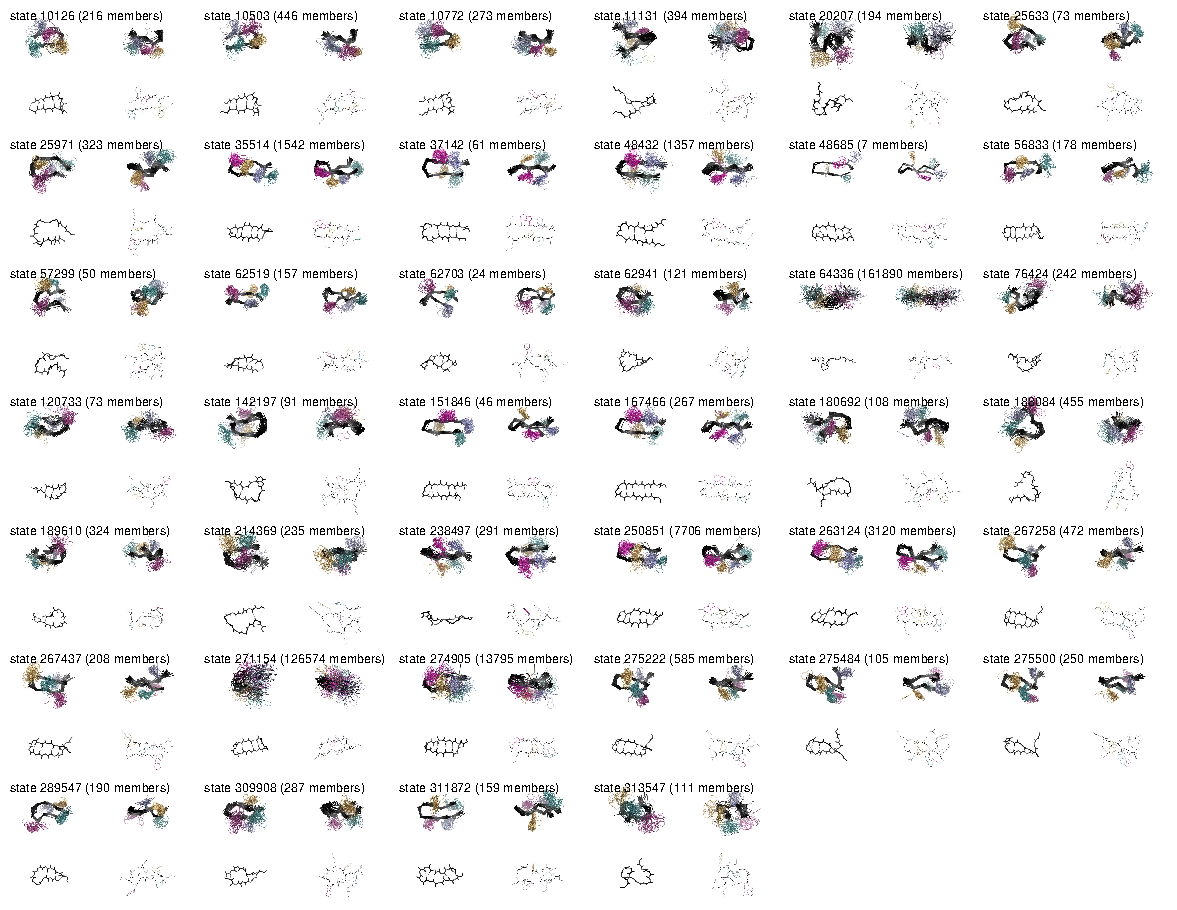
\includegraphics{chapters/automatic-state-decomposition/figures/trpzip2/trpzip2-states.pdf}}
  \end{center}
  \caption{{\bf Automatic state decomposition applied to trpzip2 to produce 40 macrostates.}}
  \label{automatic:figure:trpzip2-allstates}
\end{figure}

%\chapter{Efficient methods for computing interstate transition rates}
\label{chapter:efficient-computation-of-transition-rates}

%Because of the deficiencies observed in the ability of replica-exchange simulations to reach equilibrium, even after unpractically long simulation times (cite bill trpzip2), we are forced to resort to other means to compute equilibrium transition probabilities.
%One way to compute equilibrium expectations is through uncoupling-coupling approaches...
%\chapter{Multistage and iterative methods for the efficient and automatic construction of master equation models}
\label{chapter:automatic-construction-of-master-equation}
 

%%%%%%%%%%%%%%%%%%%%%%%%%%%%%%%%%%%%%%%%%%%%%%%%%%%%%%%%%%%%%%%%%%%%%%%%%%%%%%%%%%%%%%%%%%%%
%% CONCLUSION
%%%%%%%%%%%%%%%%%%%%%%%%%%%%%%%%%%%%%%%%%%%%%%%%%%%%%%%%%%%%%%%%%%%%%%%%%%%%%%%%%%%%%%%%%%%%
\chapter{Conclusion}
\label{chapter:conclusion}

In this dissertation, we have considered the problem of how the dynamics of biological macromolecules can be studied using discrete-state master equation or Markov models.
The construction of these models requires two elements: a way of decomposing configuration space into states, and a method for computing transition rates or probabilities among these states.
Chapter \ref{chapter:mastereqn-alanine-long-times} contained a proof of concept, demonstrating that a model constructed from short trajectories for a model system, terminally-blocked alanine peptide in explicit solvent, was capable of accurately describing the statistical dynamics over long times.
In Chapter \ref{chapter:validation-of-master-equation}, we considered a number of tests to establish the timescale at which the stochastic model would be an appropriate description of dynamics, an important prerequisite for evaluating various state decompositions.
Finally, Chapter \ref{chapter:automatic-state-decomposition} presented a first attempt at an \emph{automatic} algorithm for finding an optimal set of states given the number of states desired.
These last two chapters describe the minimal essential ingredients for the construction of these models for problems of biological interest.

There are obviously many remaining challenges before the use of these models becomes widespread, and before it is possible to tackle the most interesting questions in biology.
Currently, the quantity of data needed to construct these models requires the resources of massive computing projects, such as Blue Gene or Folding@Home, though it is becoming apparent that equilibrium datasets from these projects are also insufficient to construct well-determined Markov models.
Future work will concentrate on multistage sampling techniques.
There, an initial set of simulations is used to construct a crude state space, from which sets of trajectories are initiated.
By use of well-defined starting distributions that completely cover configuration space (\emph{e.g.}\ \cite{swope:2004a,weber-thesis:2006a,kube:2006a}), equilibrium transition probabilities can be reliably computed even if global equilibrium has never been achieved, as we saw in Chapter \ref{chapter:validation-of-master-equation}.
Alternatively, automatic algorithms to construct Markov models may start a number of simulations from any known structural information (\emph{e.g.}\ crystal structures, NMR ensembles, or homology models) and iteratively construct and update the model, continually discovering new metastable states and reapportioning computational effort to always explore the most poorly characterized regions, perhaps using a method like the one described by Singhal \emph{et al.}\ \cite{singhal:2005a}.
Transition path sampling \cite{dellago:1998b,bolhuis:2002a} could be employed to more efficiently compute transition rates or probabilities between states if at least one trajectory connecting the two has been found.

Further progress in the efficient construction of these models from biomolecular simulation data will lend insight into the biophysical processes of protein folding and dynamics.
More efficient algorithms will not only allow more complex problems to be addressed, but also will allow these models to be constructed with modest computer clusters instead of distributed computing projects.
There may come a time when the majority of molecular simulations are performed to construct these models.
After all, what good is a single trajectory when the entire statistical dynamics can be characterized instead?



%%%%%%%%%%%%%%%%%%%%%%%%%%%%%%%%%%%%%%%%%%%%%%%%%%%%%%%%%%%%%%%%%%%%%%%%%%%%%%%%%%%%%%%%%%%%
%% APPENDICES
%%%%%%%%%%%%%%%%%%%%%%%%%%%%%%%%%%%%%%%%%%%%%%%%%%%%%%%%%%%%%%%%%%%%%%%%%%%%%%%%%%%%%%%%%%%%
\appendix
%\chapter{A primer on statistical uncertainties}
\label{chapter:statistical-uncertainty-primer}

 

%%%%%%%%%%%%%%%%%%%%%%%%%%%%%%%%%%%%%%%%%%%%%%%%%%%%%%%%%%%%%%%%%%%%%%%%%%%%%%%%%%%%%%%%%%%%
% BIBLIOGRAPHY
%%%%%%%%%%%%%%%%%%%%%%%%%%%%%%%%%%%%%%%%%%%%%%%%%%%%%%%%%%%%%%%%%%%%%%%%%%%%%%%%%%%%%%%%%%%%
\bibliographystyle{plain}
\bibliography{jdcthesis}

\end{document}

